\chapter{Lemmatisation et indexation du corpus}

L'objectif de ce TD est de normaliser le vocabulaire par lemmatisation, d'affiner l'anti-dictionnaire à la lumière de cette normalisation, et de construire les fichiers inverses définitifs.

\section{Lemmatisation du corpus filtré}

\subsection{Architecture du module}

On définit une classe abstraite \texttt{Stemmer} exposant une interface commune (\texttt{make\_table}, \texttt{transform}, \texttt{transform\_tolist}, \texttt{save\_table}), dont héritent \texttt{SpacyStemmer} et \texttt{SnowStemmer}. Cette conception les rend interchangeables dans le pipeline sans modifier le code appelant.

\subsection{Implémentation des deux stemmers}

\texttt{SpacyStemmer} s'appuie sur le modèle français \texttt{fr\_core\_news\_sm}. Plutôt que de soumettre le texte brut à spaCy, on lui fournit directement les tokens produits par \texttt{CorpusTokenizer} en construisant manuellement un objet \texttt{spacy.tokens.Doc}. Cela garantit une tokenisation cohérente avec le reste du pipeline et évite tout désalignement avec l'index.

\texttt{SnowStemmer} utilise le \texttt{SnowballStemmer} de NLTK configuré pour le français. Chaque token est raciné indépendamment via \texttt{model.stem()}, sans contexte grammatical : l'approche est déterministe et rapide, mais aveugle aux nuances morphologiques.

\subsection{Analyse comparative et choix}

Le script \texttt{3-make\_stemmer\_tabs.py} applique les deux stemmers sur \texttt{nostopwords\_corpus.xml} et sauvegarde les tableaux \texttt{token}/\texttt{lemma} pour analyse. Sur notre corpus de \textbf{14 344 tokens uniques}, SpaCy produit \textbf{11 285 lemmes uniques} et Snowball \textbf{9 046 racines uniques}. La courbe de Pareto confirme que les deux approches suivent un profil similaire, avec environ 20\% des lemmes couvrant 80\% du corpus, Snowball ayant toutefois une distribution plus extrême.

La différence qualitative est plus décisive : Snowball réduit \textit{optimisation} et \textit{optimiste} à la même racine \texttt{optim}, causant des collisions sémantiques problématiques pour un moteur de recherche. \textbf{On retient SpaCy} : on perd en rappel (l'utilisateur doit être plus précis), mais on gagne en précision en évitant ces confusions.

\section{Affinage de l'anti-dictionnaire}

La lemmatisation regroupe plusieurs formes fléchies sous un même lemme, augmentant mécaniquement la fréquence de certains termes jusque-là sous le seuil. Par exemple, \textit{permettre} avait un TF-IDF moyen de 0.92 avant lemmatisation ; après, l'absorption de \textit{permet}, \textit{permettent}, \textit{permis} et \textit{permettait} fait chuter cette moyenne à 0.42. De même, \textit{son} absorbe \textit{sa}, \textit{leur} et \textit{leurs}. En maintenant le même seuil $\text{tfidf} \leq 0.7$, on élimine ces nouveaux termes sans ajuster les hyperparamètres. Le corpus doublement filtré est produit par \texttt{3-clean\_data.py}.

\section{Construction des fichiers inverses}

La classe \texttt{Index} est appliquée au corpus doublement filtré et lemmatisé. On obtient un fichier TSV par champ indexé : \texttt{index\_titre.tsv}, \texttt{index\_texte.tsv}, \texttt{index\_rubrique.tsv}, \texttt{index\_date.tsv}, \texttt{index\_auteur.tsv}, \texttt{index\_contact.tsv} et \texttt{index\_image.tsv}, chacun contenant le lemme, sa fréquence totale et la liste des identifiants d'articles associés.

La structure retenue est un dictionnaire Python offrant des recherches en $O(1)$, tout à fait adapté à la taille du corpus. Pour de plus grands corpus, des alternatives comme les \textbf{tables de hachage}, les \textbf{arbres binaires de recherche} ($O(\log n)$ garanti) ou les \textbf{B-Trees} (standard pour l'indexation sur disque) seraient envisageables.

\begin{figure}[h]
    \centering
    \hspace*{-0.12\textwidth}
    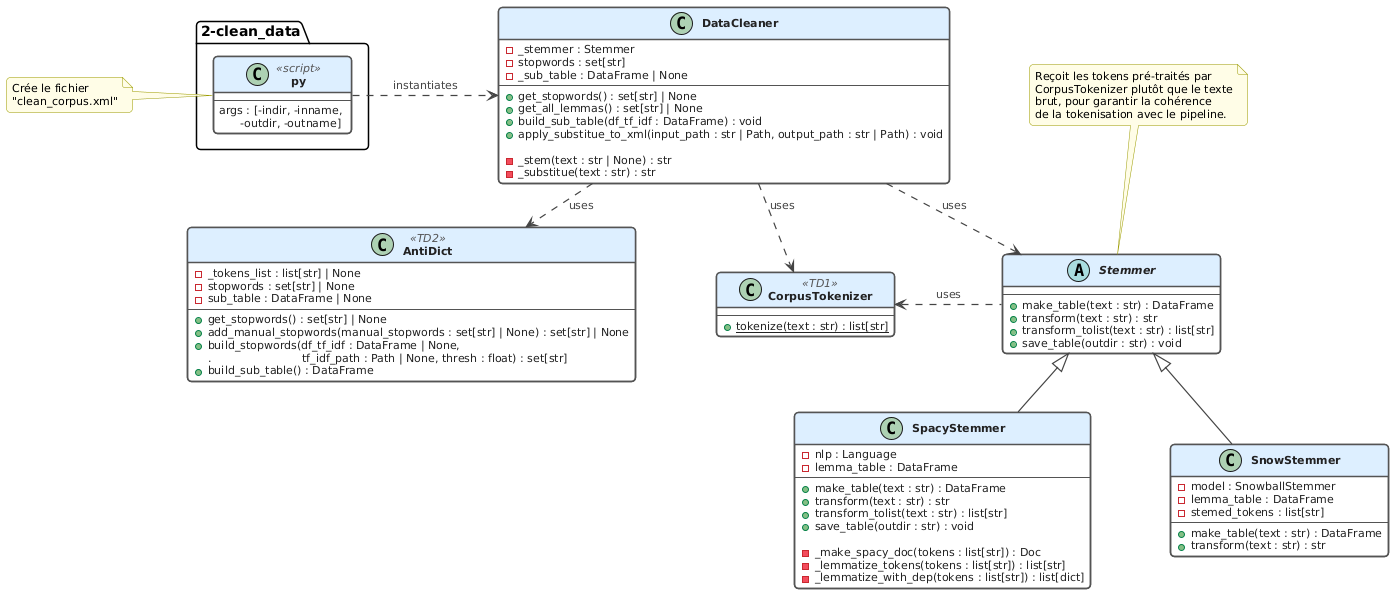
\includegraphics[width=1.2\textwidth]{assets/2-DataCleaner_AntiDict_Stemmer.png}
    \caption{UML Stemmer + AntiDict (TD1)}
    \label{fig:TD2-3-Antidict_Stemmer}
\end{figure}
